% 
%
\documentclass[12pt]{article}
% General packages
\usepackage{amsmath, graphicx, float, tabularx, booktabs, color}
% For coloring tables
%\usepackage[table]{xcolor}
% For adjusting margin size
\usepackage[margin=1in]{geometry}
% For setting bookmarks on pdf export
\usepackage[bookmarks,bookmarksopen,bookmarksdepth=2]{hyperref} 
\usepackage{cite}
\usepackage{listings}

% Image path location
\graphicspath{ {images/} }

%Define Colors
\definecolor{dkgreen}{rgb}{0,0.6,0}
\definecolor{gray}{rgb}{0.5,0.5,0.5}
\definecolor{mauve}{rgb}{0.58,0,0.82}

% Color Code
\lstset{frame=tb,
  language=ruby,
  aboveskip=3mm,
  belowskip=3mm,
  showstringspaces=false,
  columns=flexible,
  basicstyle={\small\ttfamily},
  numbers=none,
  numberstyle=\tiny\color{gray},
  keywordstyle=\color{blue},
  commentstyle=\color{dkgreen},
  stringstyle=\color{mauve},
  breaklines=true,
  breakatwhitespace=true,
  tabsize=4
}

\begin{document}

% Title information
\title{Stop and Wait Data Communication Protocol}
\author{Devin Trejo \tabularnewline devin.trejo@temple.edu}
\date{\today}
\maketitle

\section{Summary}
\label{sect:summary}
Today we introduce the stop-and-wait sliding window transmission method 
and compare the performance for difference values of window size and 
sequence size. We find that a window size that is too small decreases
performance but having a window size that is too big introduces the
probability that errors will occur during transmission. From testing
multiple parameters we find that a windows size of 04 produces the results
with the fastest transmission for our 26 packet long test message. 

\section{Introduction}
\label{sect:intro}
\subsection{Sliding Window Background}
\label{sect:background}

For this lab we will analyze and implement a sliding-window transfer
protocol between a PIC32 Server and Client application. Sliding window
flow control is an effective transfer method in which the receiver will
have a window of (\textbf{P}) frames that may be transmitted to a receiver. On
the receiver, we send ACK packets back to the sender corresponding to a 
sequence number (\textbf{M}) seen in the header of received DataPacket.  As 
ACKs come back into our reviver we move our window frame edge forward. If a 
DataPacket is lost in transmission or is corrupted once it reaches the 
receiver, the sender will attempt to re-send the DataPacket if no ACK is 
receiver within a timeout period. 

\begin{figure}[H]
    \centering
    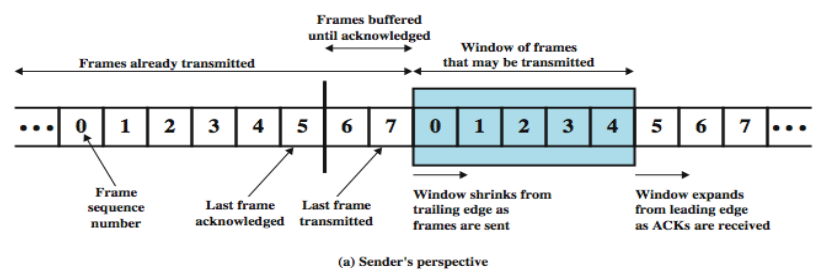
\includegraphics[width=4.5in]{slide_tx_diagram.png}
    \caption{Sliding Window Flow Control Sender}
    \label{fig:slidetx}
\end{figure}

\begin{figure}[H]
    \centering
    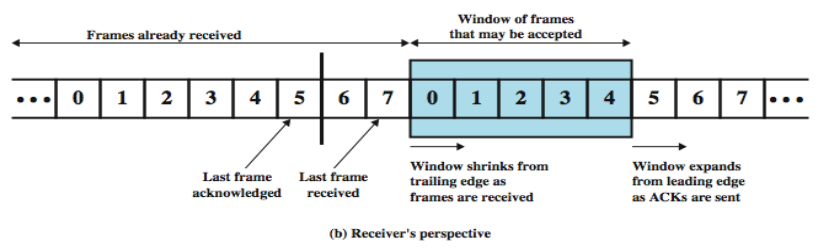
\includegraphics[width=4.5in]{slide_rx_diagram.png}
    \caption{Sliding Window Flow Control Receiver}
    \label{fig:sliderx}
\end{figure}

\subsection{Sliding Window Implementation}
\label{sect:slideimplmentation}
For this lab we implement a stop-and-wait sliding window approach which 
means we won't send the next P window until all data-packets sent in the
previous P window are acknowledged. Our data-packets are constructed to 
have a data portion size of 16 bytes and a header section containing a
single field for the 1 byte sequence number as seen in 
figure~\ref{fig:slidedatastructs}. The sender will send back ACK packets
which contain a 1 byte sequence number in the header and a 1 byte data portion
containing the ASCII ACK character as seen in figure~\ref{fig:slideackstructs}. 
We implement the protocol packet structures using structs in the C 
programming language as seen in code listing~\ref{lst:slidestructs}. 

\begin{figure}[H]
    \centering
    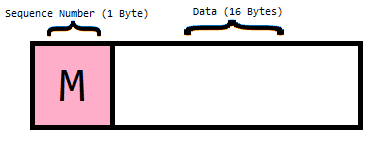
\includegraphics[height=1in]{datapacket_struct.png}
    \caption{DataPacket Structure}
    \label{fig:slidedatastructs}
\end{figure}

\begin{figure}[H]
    \centering
    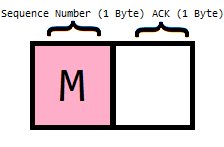
\includegraphics[height=1in]{ack_struct.png}
    \caption{ACKPacketStructure}
    \label{fig:slideackstructs}
\end{figure}

To test the protocol developed we utilize a Visual Basic Application which
will buffer and received data from the PIC32 MCU, and echo back the buffered
data after a period of \textit{X} seconds. This application allows us to develop
both client and server side message handling from the PIC32. 
To differentiate the received message from either a ACKPacket or a DataPacket 
we look at the received buffer size store in $rlen$ variable.
If the $rlen$ of the received message is a multiple of our DataPacket size
(17 bytes), we parse the message as if it were a DataPacket as seen
in code listing~\ref{lst:slidedatapacket}. Otherwise we say the received
message is a ACKPacket and parse it accordingly as seen in code 
listing~\ref{lst:slideackpacket}. 

The DataPacket message handler will mimic the role of the receiver in that
it will respond with ACKPackets to all received DataPackets. To experiment
further with the capabilities of sliding-window, we take the sequence
numbers of all received DataPackets and shuffle them. We also
will only send ACKPackets back for the corresponding received DataPackets 
with uniform probability of $PROBERR<0.1$. 

Our ACKPacket message handler will keep track of the number of ACKPackets
it received back and compare it to the original number of DataPackets it 
sent out originally. As stated by the stop-and-wait sliding window protocol,
we do not send the next P packets until all previously sent DataPackets have
been Acknowledged. Once we have received all ACKPackets, we send the next
P packets taking into account sequence number roll-over and hitting the
end of overall message transmission. 

To take into account the $PROBERR$ of not received an ACK we incorporate
a timeout feature into our stop-and-wait sliding protocol implementation. 
For all sent DataPackets we expect a corresponding ACKPacket which is 
handled by the ACKPacket message handler. If after a period of $ACKTIMEOUT$
there still hasn't been a ACK for a subset of previously sent DataPackets,
we re-transmit those DataPackets. This feature is handled by determining if
the testStarted flag is set high and delayCount has reached the timeout limit.
The process is seen in code listing~\ref{lst:slideacktimeout}.

There is a special case we also take into account for when we want to start 
our experiment, in which we detect if a global reset has been sent from the
Visual Basic application. A global reset message starts with a character
sequence of 0x0247. There would be a collision with detecting the global reset
from a DataPacket if the sequence number of the DataPacket is 0x02 and
first entry in the data field a 0x47 so we also set a $testStarted$ flag
high when the global reset has been set before. The global reset will solely
begin transmission of our data sending the P packets as defined by the user. 

\section{Discussion}
\label{sect:discussion}
\subsection{Sliding Window Testing Setup}
\label{sect:slidetest}
For testing we construct a overall message spread across 26 DataPackets. Each
packet will contain 16 bytes of which will be a corresponding letter of the 
alphabet. For example, the first DataPacket will contain a sequence number of
1 and contain 16 `A' characters within the data portion of the DataPacket. 
We will test various values for independent parameters which are show in 
table~\ref{table:independentparam}. Also of note, due to limitations
with our testing environment, (having to use a Visual Basic Application as
a middleman repeating apparatus) we package our P DataPackets into one 
larger Packet transmission. In a more traditional client/server interaction,
each one of DataPackets would be a separate transmission.

\begin{table}[H]
    \centering
    \begin{tabularx}{\textwidth}{|*{2}{>{\centering}X|}}
        \toprule
        \textbf{Parameter} & \textbf{Description} \tabularnewline
        \midrule
        \textbf{LENP} & Window Size\tabularnewline
        \textbf{LENM} & Sequence Size\tabularnewline
        \textbf{PROBERR} & Uniform Probability of Transmission Error
        \tabularnewline
        \textbf{ACKTIMEOUT} & Timeout until Re-Transmission (in MSEC)
        \tabularnewline
        \bottomrule
    \end{tabularx}
    \caption{Independent Experiment Parameters and their Descriptions}
    \label{table:independentparam}   
\end{table}

\subsection{Sliding Window Test 1}
\label{sect:slidetest1}
The parameters for this first test as seen in table~\ref{table:slidetest1}.
For the first test we will demonstrate the effectiveness of our sliding
window protocol implementation by using WireShark captures. 

\begin{table}[H]
    \centering
    \begin{tabularx}{\textwidth}{|*{2}{>{\centering}X|}}
        \toprule
        \textbf{Parameter} & \textbf{Value} \tabularnewline
        \midrule
        \textbf{LENP} & 4\tabularnewline
        \textbf{LENM} & 10\tabularnewline
        \textbf{PROBERR} & 0.5\tabularnewline
        \textbf{ACKTIMEOUT} & 5000
        \tabularnewline
        \bottomrule
    \end{tabularx}
    \caption{Sliding Window Test 1}
    \label{table:slidetest1}   
\end{table}

We begin by establishing connection between our PIC32 MCU and our Visual
Basic application. We started the test by sending the Global Reset signal
to our PIC32 which responds by sending the first 4 DataPackets to the
the Visual Basic application totaling 122 bytes. We can see our packet
data content contains the expect alphabet characters and our sequence number
ranges from 1$\rightarrow$4. 

\begin{figure}[H]
    \centering
    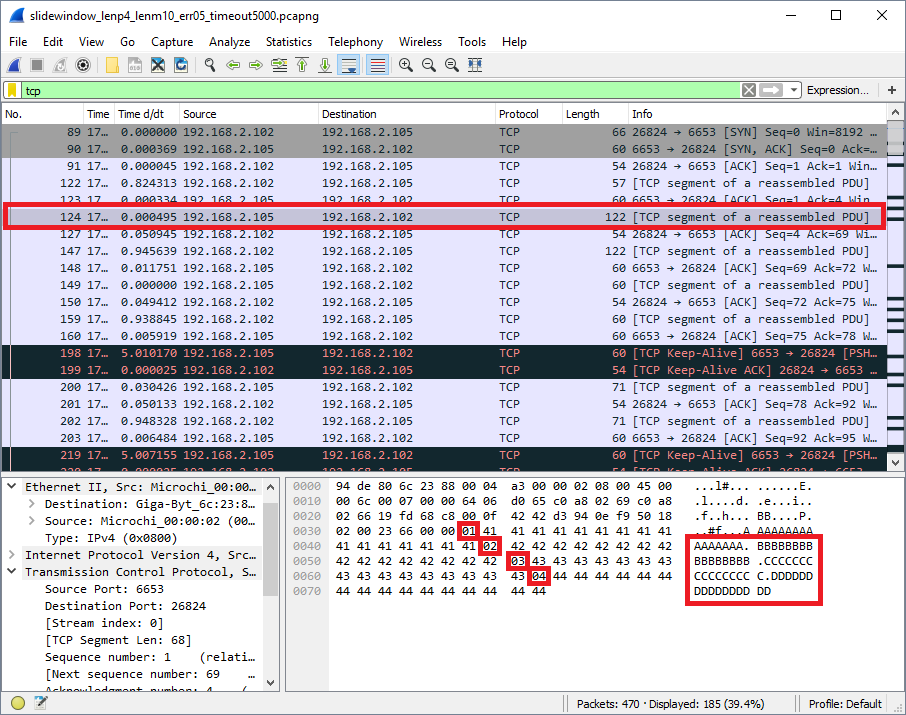
\includegraphics[width=5.5in]{slide_test1_00.png}
    \caption{Test1 - First P-Frame DataPacket Transmission}
    \label{fig:slidetest00}
\end{figure}

After a period of 0.94~seconds, our Visual Basic echos back the message to 
our PIC32. At this point our DataPacket message handler takes in the four
transmitted DataPackets and creates an ACK message for them in random order
with a uniform probability of error of 0.5. In this test run we can see
our receiver responds to three out of the four received DataPackets in a 
sequence number order of 02, 03, and 01. Missing is an ACKPacket for 04. 
Also, note the construction of the packet, containing the sequence number and
the ASCII ACK characters corresponding to HEX value 0x06.

\begin{figure}[H]
    \centering
    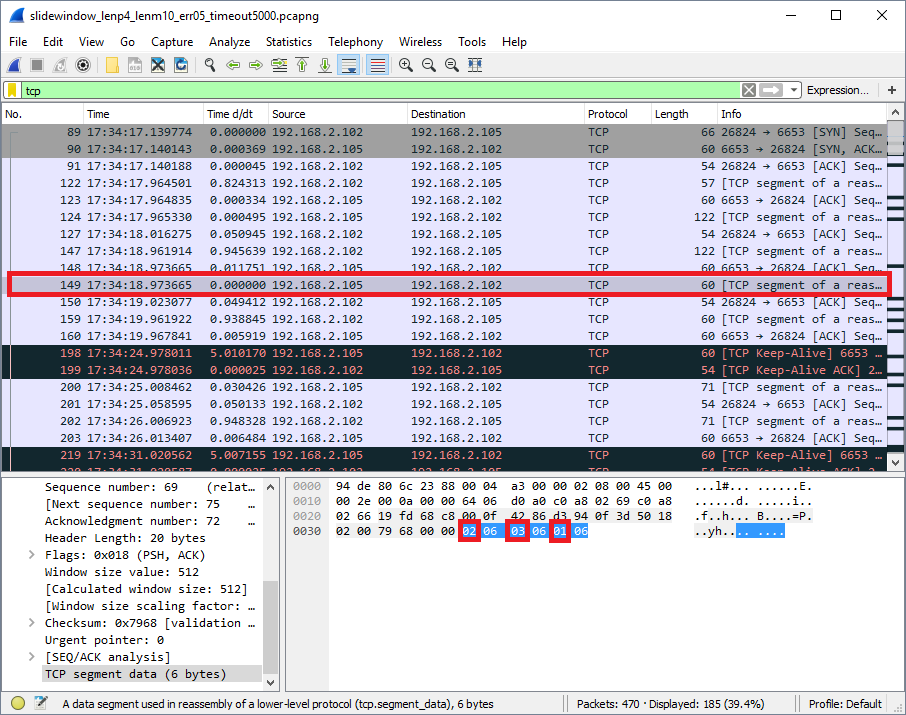
\includegraphics[width=5.5in]{slide_test1_01.png}
    \caption{Test1 - First ACKPacket for P-Frame Transmission}
    \label{fig:slidetest01}
\end{figure}

The received ACKPackets are handled by the ACKPacketHandler which tracks
the three acknowledged packets. Since not all four packets are acknowledge,
we see no transmission of the next P packets. Instead after a time period of
7~seconds (not exactly 5~seconds due to processing overhead) we see the 
re-transmission of DataPacket containing sequence number 04.

\begin{figure}[H]
    \centering
    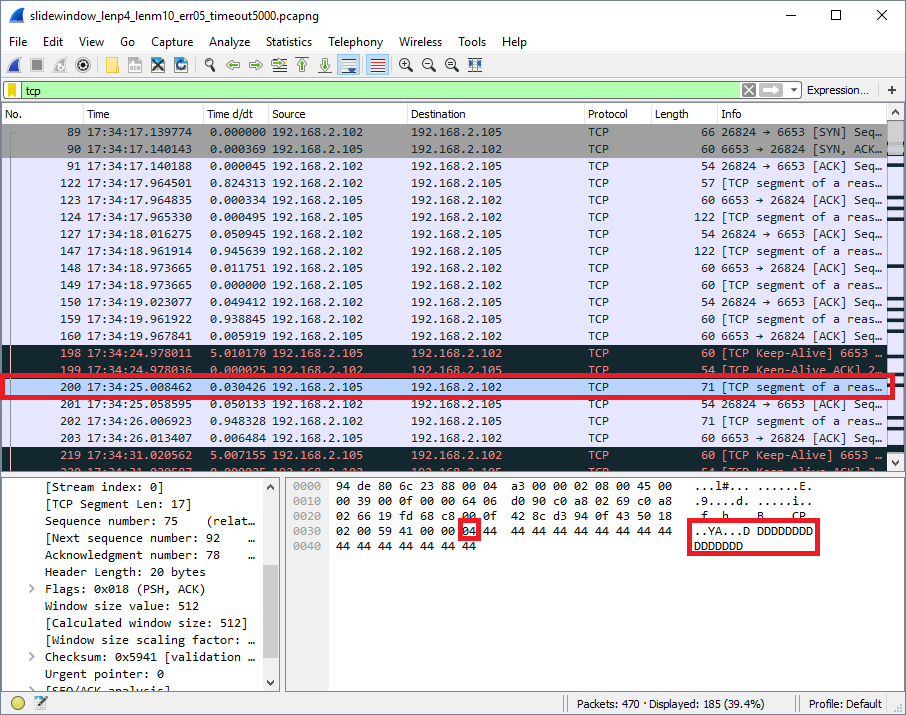
\includegraphics[width=5.5in]{slide_test1_02.png}
    \caption{Test1 - First P-Frame DataPacket Re-transmission1}
    \label{fig:slidetest02}
\end{figure}


Due to the high probability of error for this test, we again do not receive 
an ACK for this DataPacket for another 2 attempts. The transmission line 
stays silent. After each re-transmission and a time-out period of around 
5$\rightarrow$7~seconds is hit, we see another attempt of re-transmission
from our sender.

\begin{figure}[H]
    \centering
    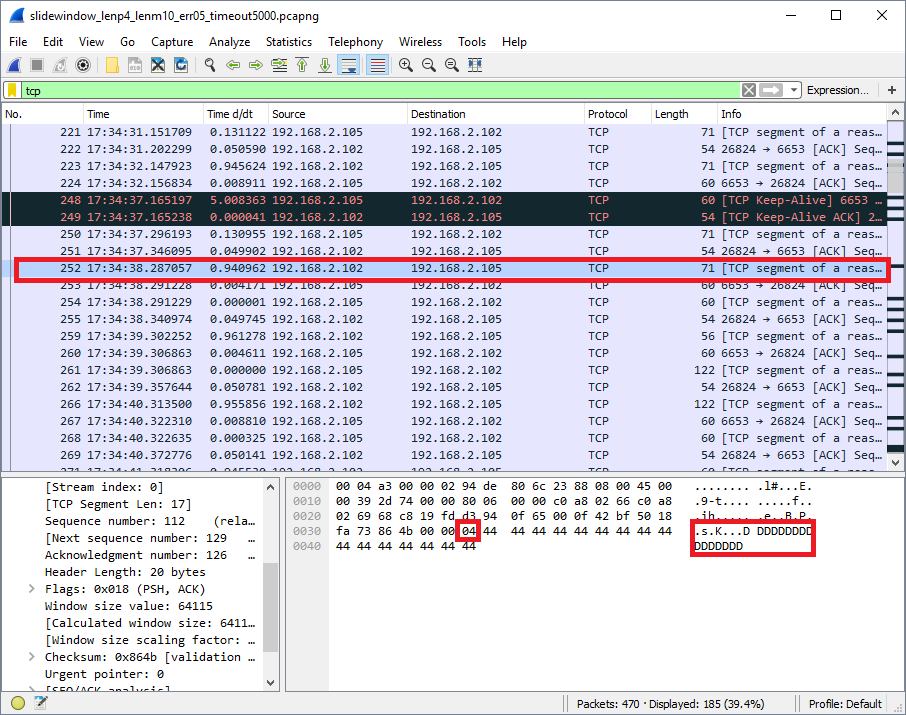
\includegraphics[width=5.5in]{slide_test1_03.png}
    \caption{Test1 - First P-Frame DataPacket Re-transmission2}
    \label{fig:slidetest03}
\end{figure}

Finally, we see a ACKPacket for sequence number DataPacket 04. 

\begin{figure}[H]
    \centering
    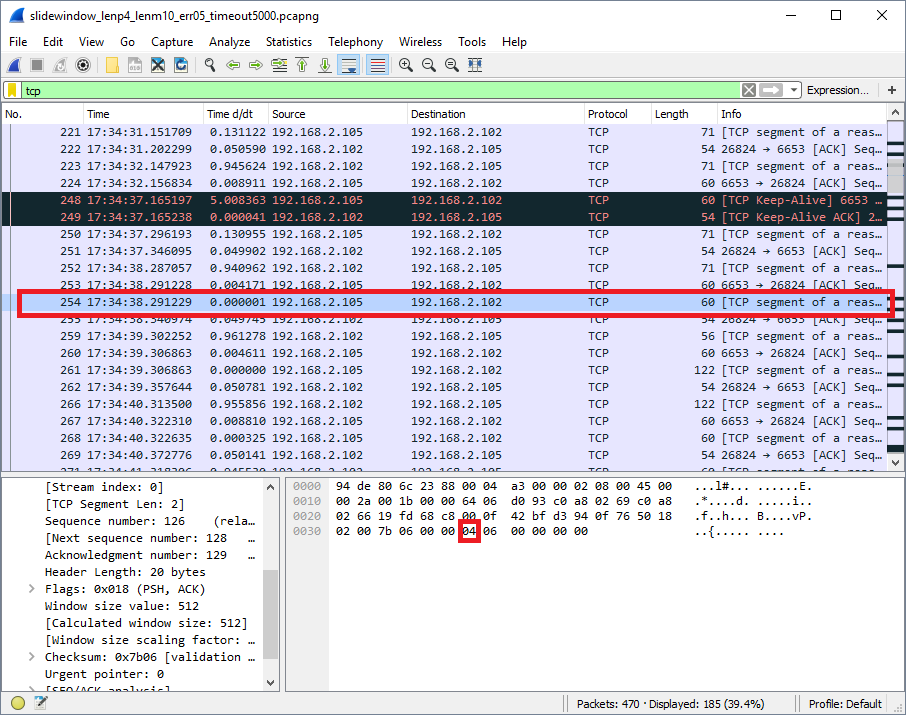
\includegraphics[width=5.5in]{slide_test1_04.png}
    \caption{Test1 - ACKPacket for DataPacket 04 Transmission}
    \label{fig:slidetest04}
\end{figure}

Shortly after receiving acknowledgment for DataPacket sequence 04, we
see transmission of the next P frame. Note the increasing sequence numbers
since we still haven't reached our sequence number rollover. 

\begin{figure}[H]
    \centering
    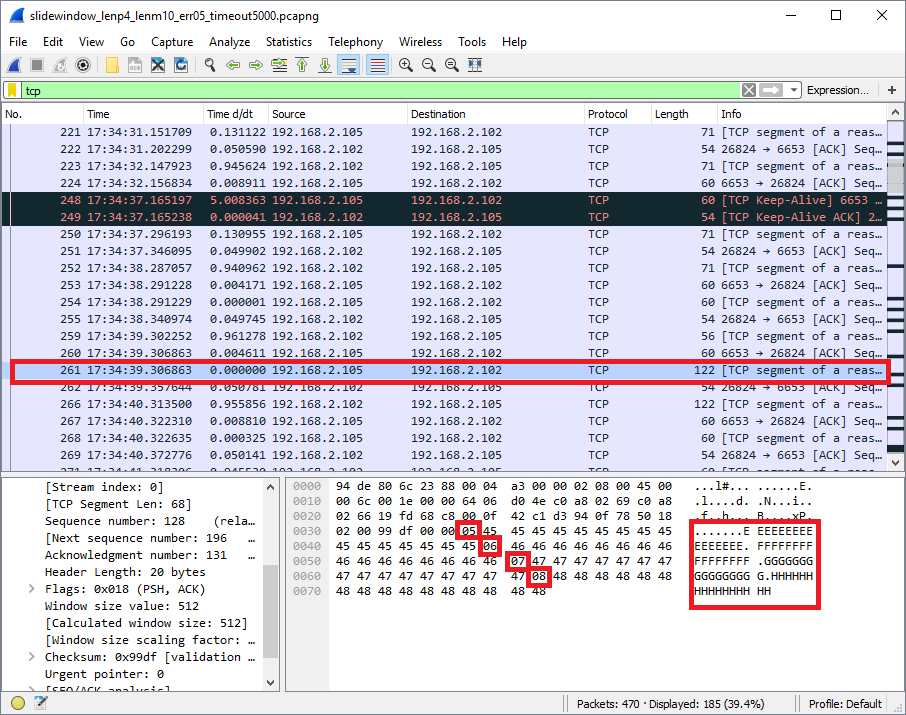
\includegraphics[width=5.5in]{slide_test1_05.png}
    \caption{Test1 - Second P-Frame DataPacket Transmission}
    \label{fig:slidetest05}
\end{figure}

The process of ACKPacket send/receive and timeout re-transmission continues
on for the full length of our 26 part message. It can be seen in 
figure~\ref{fig:slidetest06} that our sequence number rolls over. We also
see in figure~\ref{fig:slidetest07} that the full 26 part message is 
eventually fully and successfully transfered. 

\begin{figure}[H]
    \centering
    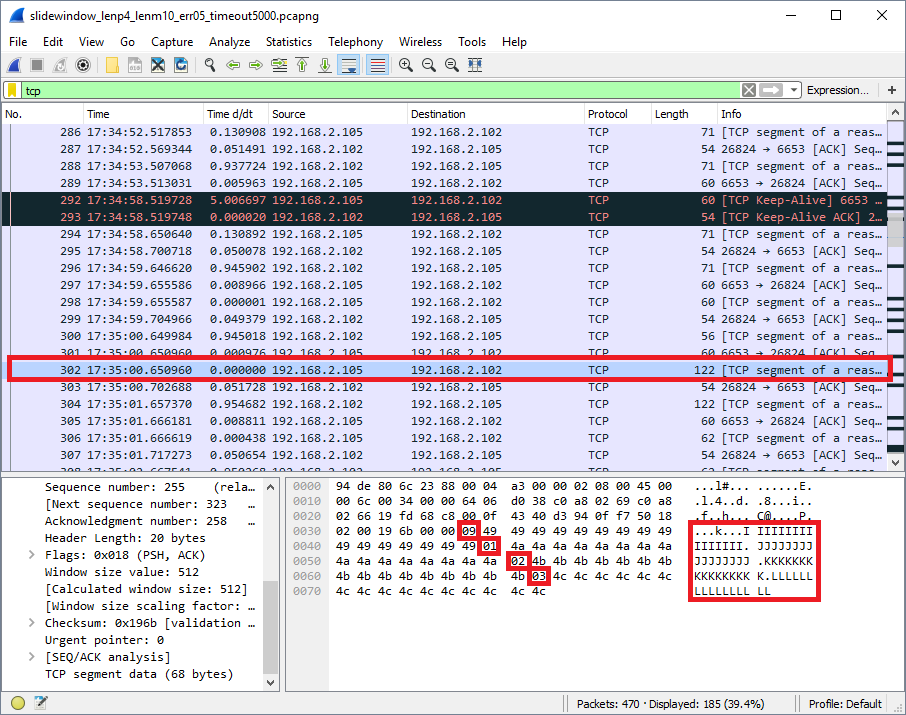
\includegraphics[width=5.5in]{slide_test1_06.png}
    \caption{Test1 - Third P-Frame DataPacket Transmission}
    \label{fig:slidetest06}
\end{figure}

\begin{figure}[H]
    \centering
    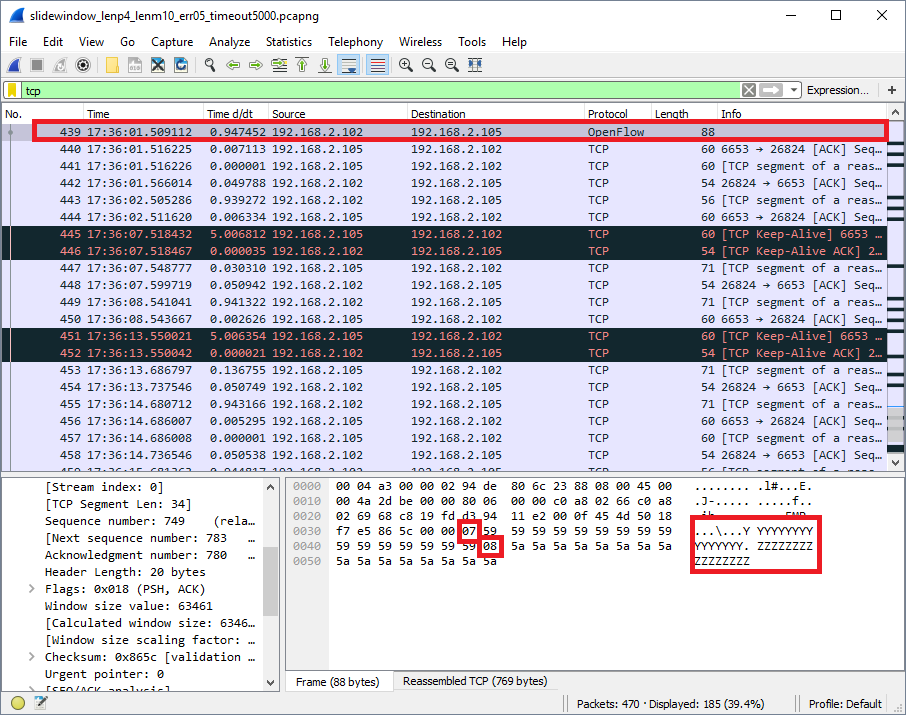
\includegraphics[width=5.5in]{slide_test1_07.png}
    \caption{Test1 - Last P-Frame DataPacket Transmission}
    \label{fig:slidetest07}
\end{figure}

Tabulated results for runtime for the combination of input parameters are
given table~\ref{table:slidetest1perf} averaged across 5 different runs.

\begin{table}[H]
    \centering
    \begin{tabularx}{\textwidth}{|*{2}{>{\centering}X|}}
        \toprule
        \textbf{Avg Runtime} &  1min 58secs\tabularnewline
        \textbf{Avg Re-Transmission Count} & 21\tabularnewline
        \bottomrule
    \end{tabularx}
    \caption{Sliding Window Test 1 - Performance}
    \label{table:slidetest1perf}   
\end{table}

\subsection{Sliding Window Test 2}
\label{sect:slidetest1}
Next we decrease our uniform probability of error and re-run our tests. 

\begin{table}[H]
    \centering
    \begin{tabularx}{\textwidth}{|*{2}{>{\centering}X|}}
        \toprule
        \textbf{Parameter} & \textbf{Value} \tabularnewline
        \midrule
        \textbf{LENP} & 4\tabularnewline
        \textbf{LENM} & 10\tabularnewline
        \textbf{PROBERR} & 0.1\tabularnewline
        \textbf{ACKTIMEOUT} & 5000
        \tabularnewline
        \bottomrule
    \end{tabularx}
    \caption{Sliding Window Test 2}
    \label{table:slidetest2}   
\end{table}

Tabulated results for runtime for the combination of input parameters are
given table~\ref{table:slidetest2perf} averaged across 5 different runs.

\begin{table}[H]
    \centering
    \begin{tabularx}{\textwidth}{|*{2}{>{\centering}X|}}
        \toprule
        \textbf{Avg Runtime} &  28secs\tabularnewline
        \textbf{Avg Re-Transmission Count} & 2\tabularnewline
        \bottomrule
    \end{tabularx}
    \caption{Sliding Window Test 2 - Performance}
    \label{table:slidetest2perf}   
\end{table}

\subsection{Sliding Window Test 3}
\label{sect:slidetest1}
Next we increase our window size from the previous test and re-run the 
experiment. 

\begin{table}[H]
    \centering
    \begin{tabularx}{\textwidth}{|*{2}{>{\centering}X|}}
        \toprule
        \textbf{Parameter} & \textbf{Value} \tabularnewline
        \midrule
        \textbf{LENP} & 7\tabularnewline
        \textbf{LENM} & 10\tabularnewline
        \textbf{PROBERR} & 0.1\tabularnewline
        \textbf{ACKTIMEOUT} & 5000
        \tabularnewline
        \bottomrule
    \end{tabularx}
    \caption{Sliding Window Test 3}
    \label{table:slidetest3}   
\end{table}

Tabulated results for runtime for the combination of input parameters are
given table~\ref{table:slidetest3perf} averaged across 5 different runs.

\begin{table}[H]
    \centering
    \begin{tabularx}{\textwidth}{|*{2}{>{\centering}X|}}
        \toprule
        \textbf{Avg Runtime} &  36secs\tabularnewline
        \textbf{Avg Re-Transmission Count} & 4\tabularnewline
        \bottomrule
    \end{tabularx}
    \caption{Sliding Window Test 3 - Performance}
    \label{table:slidetest3perf}   
\end{table}

\subsection{Sliding Window Test 4}
\label{sect:slidetest1}
The last test decreases our window size to 1.

\begin{table}[H]
    \centering
    \begin{tabularx}{\textwidth}{|*{2}{>{\centering}X|}}
        \toprule
        \textbf{Parameter} & \textbf{Value} \tabularnewline
        \midrule
        \textbf{LENP} & 1\tabularnewline
        \textbf{LENM} & 10\tabularnewline
        \textbf{PROBERR} & 0.1\tabularnewline
        \textbf{ACKTIMEOUT} & 5000
        \tabularnewline
        \bottomrule
    \end{tabularx}
    \caption{Sliding Window Test 4}
    \label{table:slidetest4}   
\end{table}

Tabulated results for runtime for the combination of input parameters are
given table~\ref{table:slidetest4perf} averaged across 5 different runs.

\begin{table}[H]
    \centering
    \begin{tabularx}{\textwidth}{|*{2}{>{\centering}X|}}
        \toprule
        \textbf{Avg Runtime} & 57secs\tabularnewline
        \textbf{Avg Re-Transmission Count} & 7\tabularnewline
        \bottomrule
    \end{tabularx}
    \caption{Sliding Window Test 4 - Performance}
    \label{table:slidetest4perf}   
\end{table}

\section{Conclusion}
\label{sect:conclusion} 
In conclusion, we found see that to best utilize the available bandwidth
of your transmission line it is best to break your message into smaller 
message sizes. Doing so, ensures that you are utilizing the available 
bandwidth and minimizes the need for re-transmission since corruption of 
smaller packets is less likely. There is a sweet balance between window
size that eliminates unnecessary re-transmissions but also reduces the probability
of data corruption. 

A better implementation of the sliding window approach would be selective 
reject. Selective reject is the process for the sender to request specific
frames that it has failed to received or that have been received but corrupted.
The process can ride along our stop-and-wait ACKPacket already implemented in
this experiment but instead of only sending ASCII ACK characters we send 
ASCII NAK that tells the sender to retransmit a specific frame. 
It eliminates the need for the $ACKTIMEOUT$ to catch all transmission errors.
We could also add error correction coding that would reduce need for 
re-transmission of all corrupted frames. Overall, we see that there is a 
sweet balance in transmission technique that is specific to the application
at hand. 

%\bibliographystyle{plain}
%\bibliography{}

\section*{Appendix}
\label{sect:appendix}

Main program source code available on my GitHub: \\
\url{https://github.com/dtrejod/myece4532/blob/master/lab5}

\begin{lstlisting}[language=c, 
caption=DataPacket | ACK-Packet Data Structure,
label=lst:slidestructs]
// ACK Struct
struct myACK
{
    uint8_t sequence;
    char ackChar;
};

// WARNING IF myDataPacket length and myACKs are multiples of one another,
// the packet detection algo will fail. 
struct myDataPacket 
{
    uint8_t sequence;
    char data[DATALEN];
};
\end{lstlisting}

\begin{lstlisting}[language=c, 
caption=Sliding Window - Global Reset Handler,
label=lst:slidereset]
// Check to see if message begins with
// '0271' signifying message is a global reset
// We use this as a signal to start the lab
// experiment. 
if ((testStarted == 0) && (rbfrRaw[0] == 02) && 
        (rbfrRaw[1] == 71))
{                        
    // Reset Frame Sent Variables
    tbfrDataTrackerI = 0;
    tbfrAckTrackerI = 0;

    // Reset Sequence Number
    tbfrSeqTracker = 1;

    // Reset total msg sent counter
    msgSent = 0;
    testStarted = 1;

    for(tbfrDataTrackerI=0; tbfrDataTrackerI < LENP; 
        tbfrDataTrackerI++)
    {
        // Check for seq rollover
        if(tbfrSeqTracker >= LENM)
        {
            tbfrSeqTracker = 1;
        }

        // Adjust offset
        if(tbfrDataTrackerI==0) offset=msgSent;
        // Populate sequence number
        tbfrData[tbfrDataTrackerI+offset].sequence = 
            tbfrSeqTracker++;

        // We keep track of the seq numbers we do send
        tbfrDataTracker[tbfrDataTrackerI] = 
            tbfrData[tbfrDataTrackerI+offset].sequence;

        // Copy tbfr over to 
        tbfr[tbfrDataTrackerI] = 
            tbfrData[tbfrDataTrackerI+offset];

        // Keep track of how much of the msg has been
        // sent
        msgSent++;

        if (msgSent > MSGLEN)
        {
            break;
        } 
    }
    mPORTDClearBits(BIT_0);
    mPORTDSetBits(BIT_2);   // LED3=1
    send(clientSock, tbfr, 
        sizeof(struct myDataPacket)*tbfrDataTrackerI, 0);
    mPORTDClearBits(BIT_2); // LED3=0
    DelayMsec(100);
}
\end{lstlisting}


\begin{lstlisting}[language=c, 
caption=Sliding Window - Data Packet Detector and Handler,
label=lst:slidedatapacket]
// Check what time of message was revived based on its
// size
// Check if received is an myDataPacket
if (rlen%sizeof(struct myDataPacket)==0)
{
    i=0;
    // Reset data packets received
    rbfrDataTrackerI = 0;
    
    // Parse the receive buffer until end of buffer
    while (sizeof(struct myDataPacket)*i < rlen)
    {
        // Convert the received data into a dataPacket 
        // struct
        rbfrData = (struct myDataPacket *) rbfrRaw+(i++);
        // Retrieve sequence number and store
        rbfrDataTracker[rbfrDataTrackerI++] = 
            rbfrData->sequence;
    }
    // Shuffle order of rbfrDataTracker ACKs we will send 
    // back
    shuffle(rbfrDataTracker, rbfrDataTrackerI);
    
    j=0;
    // Set sequence number P to zero and send LENP packets
    for(i=0; i < rbfrDataTrackerI; i++)
    {
        // Send ACK for Random number of packets
        if (randMToN(0.0,1.0) >= PROBERR)
        {
            rbfrAck[j].sequence = rbfrDataTracker[i];
            rbfrAck[j].ackChar = 0x06;
            j++;
        }
    }
    mPORTDClearBits(BIT_0);
    mPORTDSetBits(BIT_2);   // LED3=1
    send(clientSock, rbfrAck, 
        sizeof(struct myACK)*j, 0);
    mPORTDClearBits(BIT_2); // LED3=0
    DelayMsec(100);
}
\end{lstlisting}

\begin{lstlisting}[language=c, 
caption=Sliding Window - ACK Packet Detector and Handler,
label=lst:slideackpacket]
else if (rlen%sizeof(struct myACK)==0)
{
    // Randomize the 
    // Parse the receive buffer for myACK until end of
    // buffer
    i=0;
    while (sizeof(struct myACK)*i < rlen)
    {
        // Convert the received data into a myAck struct
        tbfrAck = (struct myACK *) rbfrRaw+(i++);
        
        // Retrieve sequence number and store
        tbfrAckTracker[tbfrAckTrackerI++] = 
            tbfrAck->sequence;
    }
    // Check if we recieved all the frames we orignally
    // sent. If yes transfer the next M frames
    if (tbfrAckTrackerI >= tbfrDataTrackerI)
    {
        if (msgSent > MSGLEN)
        {
            testStarted=0;
        }
        else 
        {
            // Check if there are more frames to send
            // Reset Frame Sent Variables
            tbfrAckTrackerI = 0;

            for(tbfrDataTrackerI=0; tbfrDataTrackerI < LENP; 
                tbfrDataTrackerI++)
            {
                // Check for seq rollover
                if(tbfrSeqTracker >= LENM)
                {
                    tbfrSeqTracker = 1;
                }

                // Adjust offset
                if(tbfrDataTrackerI==0) offset=msgSent;
                // Populate sequence number
                tbfrData[tbfrDataTrackerI+offset].sequence = 
                    tbfrSeqTracker++;

                // We keep track of the seq numbers we do send
                tbfrDataTracker[tbfrDataTrackerI] = 
                    tbfrData[tbfrDataTrackerI+offset].sequence;

                // Copy tbfr over to 
                tbfr[tbfrDataTrackerI] = 
                    tbfrData[tbfrDataTrackerI+offset];

                // Keep track of how much of the msg has been
                // sent
                msgSent++;

                if (msgSent > MSGLEN)
                {
                    break;
                }
            }
            mPORTDClearBits(BIT_0);
            mPORTDSetBits(BIT_2);   // LED3=1
            send(clientSock, tbfr, 
                sizeof(struct myDataPacket)*tbfrDataTrackerI, 0);
            mPORTDClearBits(BIT_2); // LED3=0

            DelayMsec(100);
        }
    }
}      
\end{lstlisting}

\begin{lstlisting}[language=c, 
caption=Sliding Window - ACK Timeout Handler,
label=lst:slideacktimeout]
// If rlen is zero length we increment delay count
else if (testStarted == 1)
{
    DelayMsec(10);
    delayCount++;
    
    // Check for ACK timeout
    if (delayCount*10 > ACKTIMEOUT)
    {
        // Retransmit any packets we haven't received ACKs back
        // for yet
        delayCount = 0;

        // Reset selective repeat
        selectiveRepeat = 0;

        // Set sequence number P to zero and send LENP 
        // packets
        for(i=0; i < tbfrDataTrackerI; i++)
        {
            flag = 0;
            for(j=0; j< tbfrAckTrackerI; j++)
            {
                if(tbfrDataTracker[i]==tbfrAckTracker[j])
                {
                    flag = 1;
                    break;
                }
            }
            if (flag == 0)
            {
                tbfr[selectiveRepeat++] = tbfr[i];
            }
        }
        mPORTDClearBits(BIT_0);
        mPORTDSetBits(BIT_2);   // LED3=1
        send(clientSock, tbfr, 
            sizeof(struct myDataPacket)*selectiveRepeat, 0);
        mPORTDClearBits(BIT_2); // LED3=0 
        DelayMsec(100);              
    }
}
\end{lstlisting}

\end{document}